\chapter{ПРАКТИЧЕСКАЯ РАБОТА № 3 <<МЕТОДОЛОГИЯ ФУНКЦИОНАЛЬНОГО МОДЕЛИРОВАНИЯ АРХИТЕКТУРЫ ИС>>}

\section{Цель работы}

Работа направлена на ознакомление с методологиями функционального моделирования IDEF0 и IDEF3, получение навыков по применению данных методологий для построения функциональных моделей на основании требований к информационной системе. В ходе выполнения работы необходимо выполнить обследование объекта автоматизации и составить обоснование необходимости создания ИС, согласно ГОСТ 34.601-90, выполнить анализ рисков, ознакомиться с основными методами и средствами для реализации и документирования аналитического отчета по проектированию ИС.

\section{Постановка задачи}

Выполнить проектировании следующей системы.

Предприятие занимается производством строительных материалов различных видов (цемент, кирпич, шифер, бетонные блоки). После выпуска партии готовой продукции, она передается на склад. Со склада производится отгрузка готовой продукции покупателю. При возникновении производственного брака, оформляется списание готовой продукции. Если продукция используется для производства нового изделия, ее возвращают со склада на переработку.

\section{Видение проекта}

Основными целями создания программного продукта для предприятия, занимающегося производством строительных материалов, являются:

\begin{enumerate}
	\item{Увеличение оборота предприятия за счет повышения продаж в дигитальной сфере.}
	\item{Снижение объемов потери за счет введения электронной системы учета строительных материалов различных видов.}
\end{enumerate}

К проектным ограничениям можно отнести:

\begin{enumerate}
	\item{Мощности ЭВМ предприятия ограничены, на большинстве ЭВМ сотрудников предприятия установлено проприетарное ПО --- оплата лицензий ПО превышает 5 \% дохода.}

	\item{Временные затраты на разработку зависят от пика продаж строительства на рынке --- программная система дожна быть реализована в период между II и IV кварталом текущего года.}

	\item{Помимо этого, бюджет на разработку ограничен и не может превышать 25000 USD, также средства необходимо направить на обучение работников цифровым навыкам.} 

\end{enumerate}

\section{Отчёт об обследовании предприятия}

\subsection{Организационная структура объекта}

\subsubsection{Итоговое словесное описание}

Организационную структуру можно представить следующим образом:

Главную должность в структуре объекта занимает генеральный директор, ему непосредственно подчиняются производственный отдел, складской отдел и бухгалтерия.

У начальника производственного отдела в подчинении отдел переработки и отдел готовых продуктов.

У начальника складского отдела в подчинении отдел логистики и рабочий состав склада.

\subsubsection{Схема}

На рисунке 3.1 представлена оргструктура объекта.

\begin{figure}[h!]
        \centering
        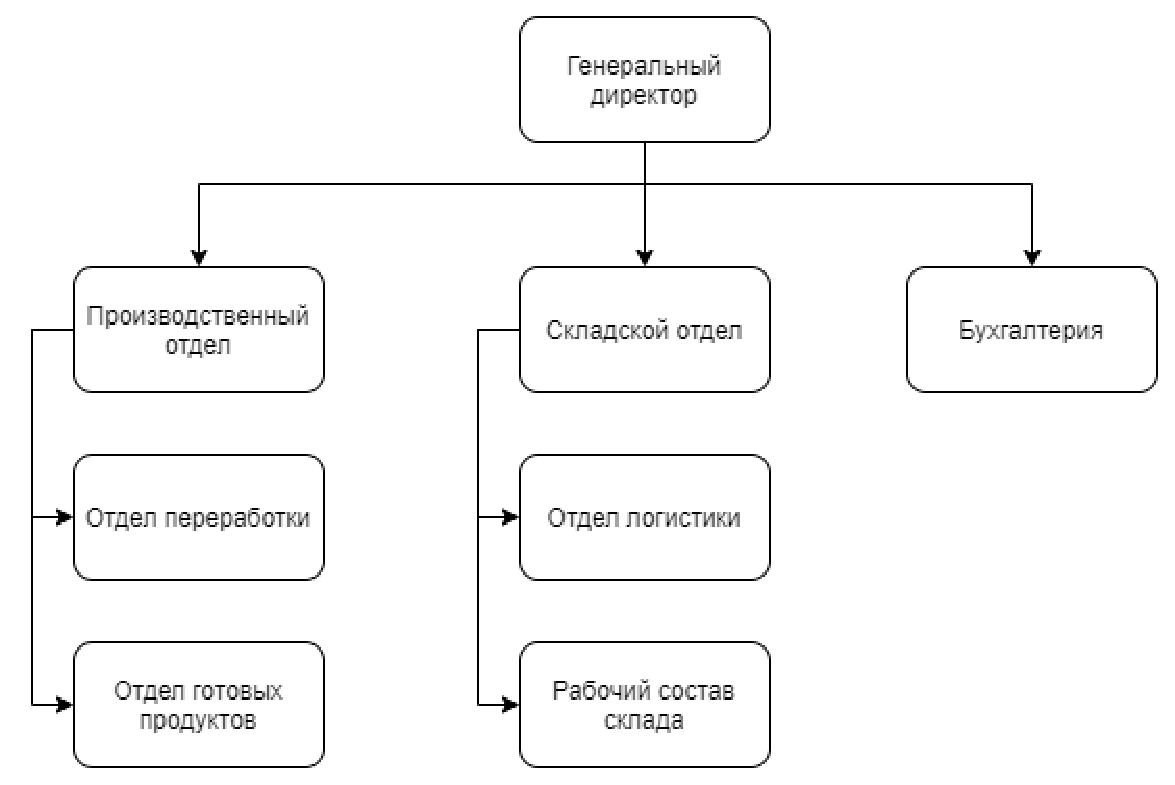
\includegraphics[width=0.5\textwidth]{images/3/hierarchy.eps}
        \caption{Организационная структура объекта}
\end{figure}

\subsection{Кадровая структура объекта}

\subsubsection{Итоговое словесное описание}

\emph{Вертикальные связи.}

Генеральному директору подчиняются начальник завода, начальник складского отдела, главный бухгалтер.

Начальнику завода подчиняется начальник смены.

Начальнику смены подчинются рабочие.

Начальнику складского отдела подчиняются главный логист и начальник склада.

Главному логисту подчиняется водитель фуры.

Начальнику склада подчиняется работник склада.

Главному бухгалтеру подчиняются бухалтеры.

\emph{Горизонтальные связи.}

Уровень 1.

Между собой взаимодействуют начальник завода, начальник складского отдела и главный бухгалтер.

Уровень 2.

Между собой взаимодействуют начальник смены, главный логист, начальник склада и бухгалтеры.

\subsubsection{Схема}

На схеме ниже представлена кадровая структура объекта.

\begin{figure}[h!]
        \centering
        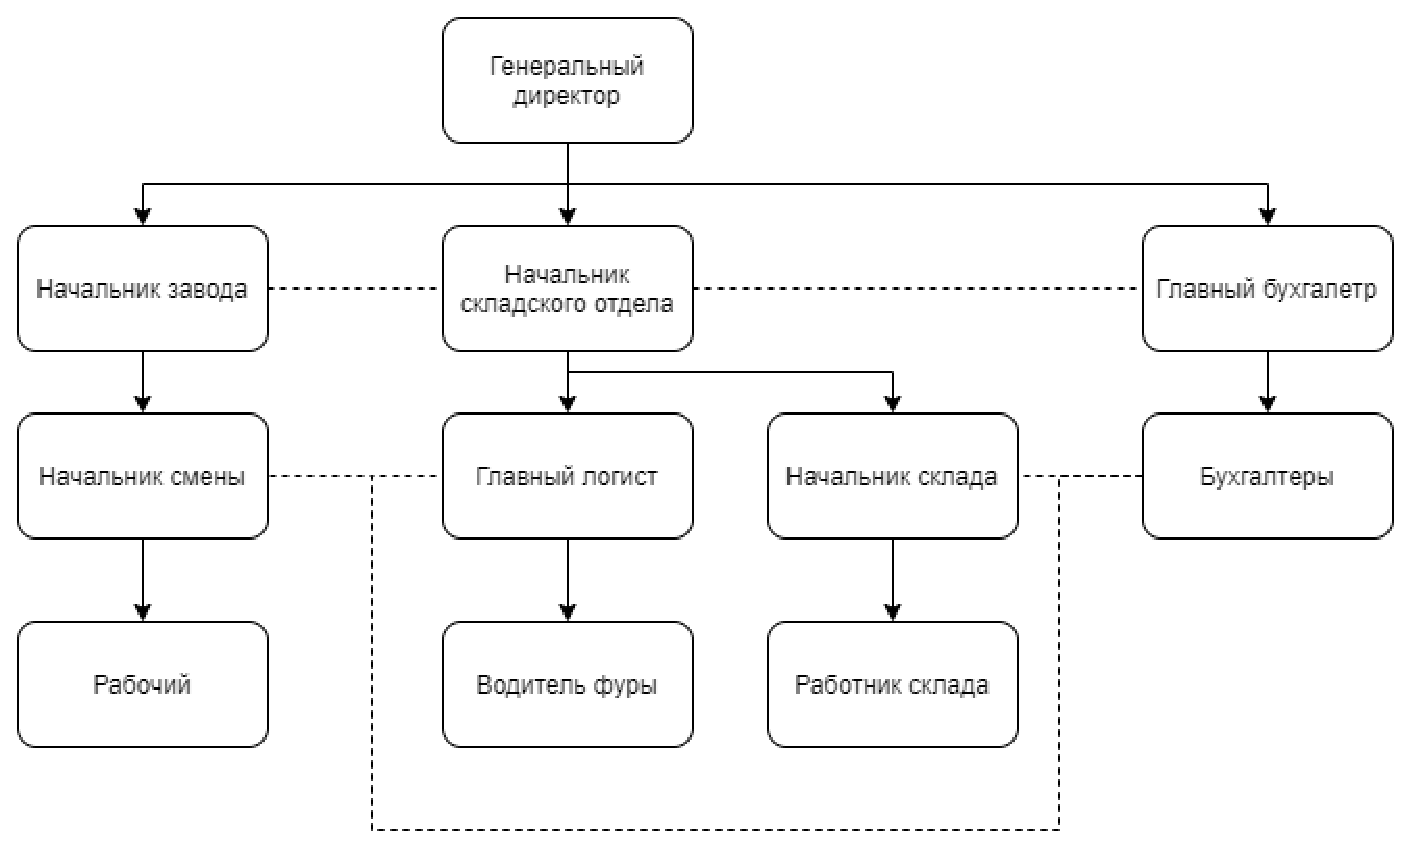
\includegraphics[width=0.5\textwidth]{images/3/hr.eps}
	\caption{Кадровая структура объекта}
\end{figure}

\subsection{Основные бизнес-процессы объекта}

\subsubsection{Итоговое словесное описание}

Основные бизнес-процессы объекта:

\begin{enumerate}

	\item{Отгрузка материалов со склада.}
	\item{Создание продуктов.}
	\item{Отгрузка на склад.}
	\item{Отгрузка покупателю.}
	\item{Оформление договора купли-продажи.}
	\item{Переработка брака.}

\end{enumerate}

	\emph{Отгрузка материалов со склада.}

	Нормативные документы --- техника безопасности.  Вход --- заявка на производство.  Выход --- материалы.  Исполнитель --- работник склада.

	\emph{Создание продуктов.}


	Нормативные документы --- техника безопасности.  Вход --- материалы.  Выход --- готовая партия.  Исполнитель --- рабочие завода.

	\emph{Отгрузка на склад.}


	Нормативные документы --- техника безопасности.  Вход --- готовая партия.  Выход --- накладная.  Исполнитель --- работник склада.

	\emph{Отгрузка покупателю.}

	Нормативные документы --- техника безопасности и законы России.  Вход --- заявка на производство.  Выход --- список отгруженных товаров.  Исполнитель --- работник склада.

	\emph{Оформление договора купли-продажи.}

	Нормативные документы --- законы России.  Вход --- список отгруженных товаров.  Выход --- чек сделки.  Исполнитель --- бухгалтерв.

	\emph{Переработка брака.}

	Нормативные документы --- техника безопасности.  Вход --- партия для переработки.  Исполнитель --- рабочие завода.

\newpage
\subsubsection{Схема}

На схеме ниже представлены основные бизнес-процессы объекта.

\begin{figure}[h!]
        \centering
        \includegraphics[width=0.7\textwidth]{images/3/business.eps}
	\caption{Основные бизнес-процессы объекта}
\end{figure}

\subsection{Декомпозиция основных бизнес-процессов объекта}

Декомпозиция процесса отгрузки на склад.

\emph{Расфасовка в доставочные блоки.}

Нормативные документы --- техника безопасности.  Вход --- готовая партия.  Выход --- упакованный товар.  Исполнитель --- работники склада.

\emph{Распределение по складу.}

Нормативные документы --- техника безопасности.  Вход --- упакованный товар.  Выход --- новые поступления на склад.  Исполнитель --- работники склада.

\emph{Оформление новых товаров на складе.} 

Нормативные документы --- законы РФ. Вход --- поступление на склад. Выход --- накладная. Исполнитель --- работники склада.

\subsubsection{Схема}
\begin{figure}[h!]
        \centering
        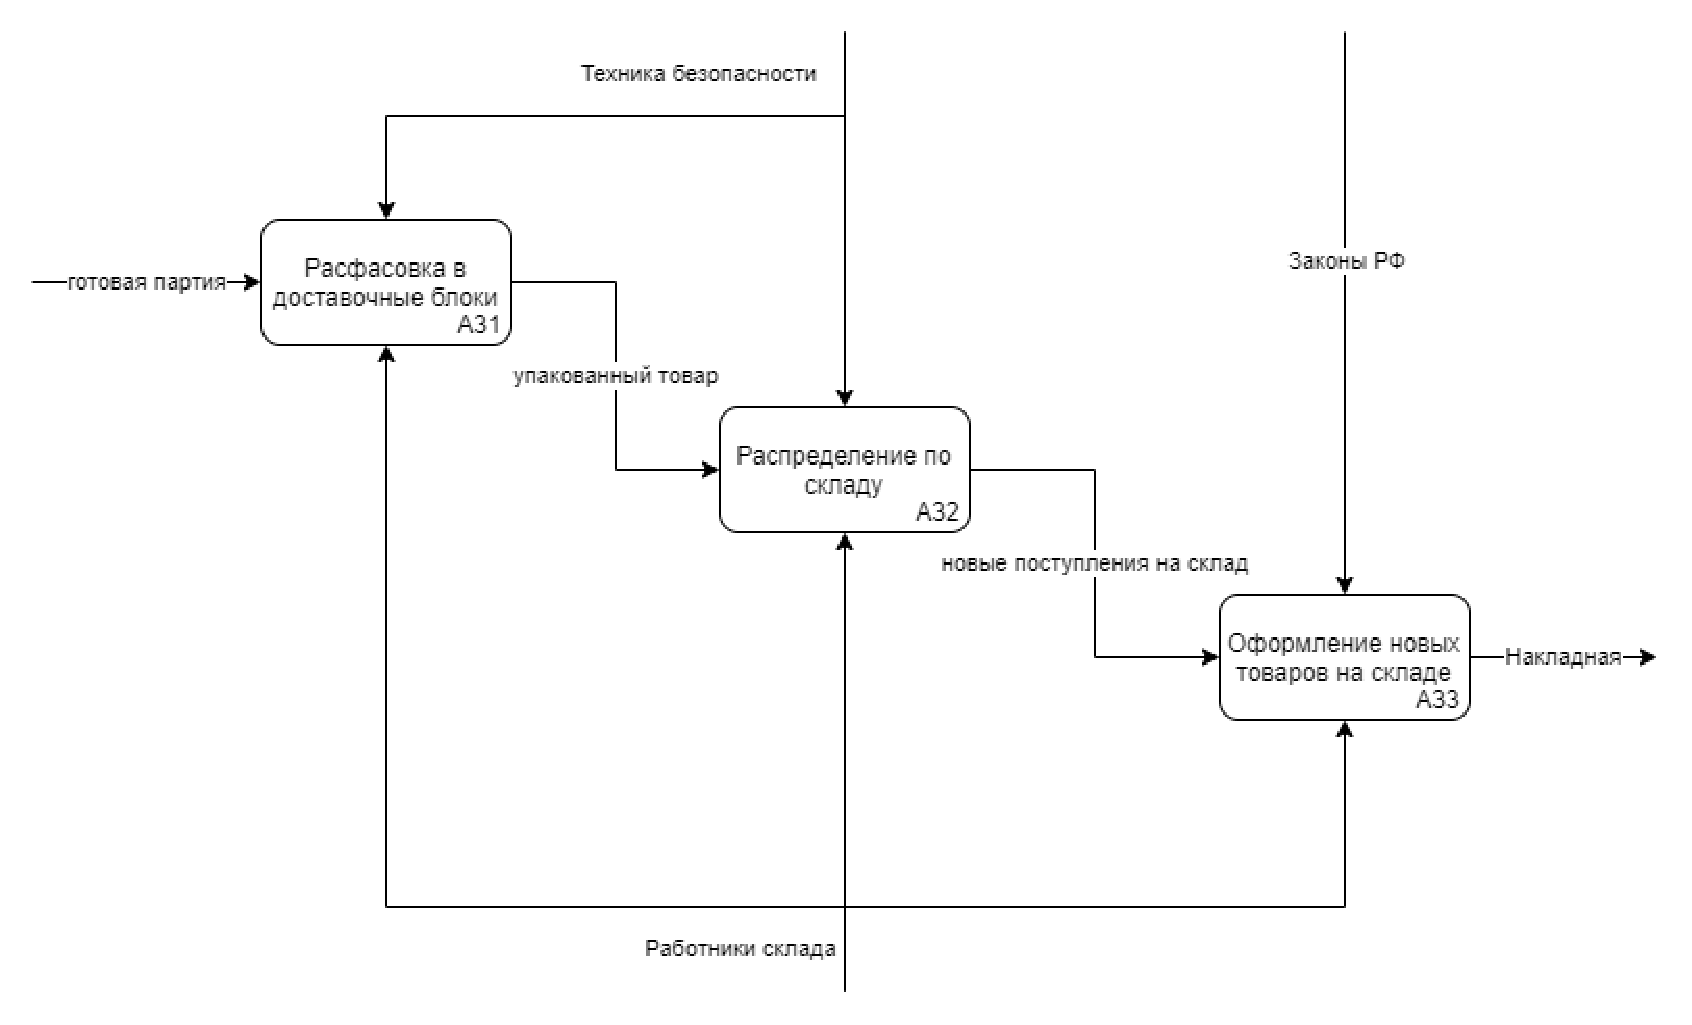
\includegraphics[width=0.8\textwidth]{images/3/decompose.eps}
	\caption{Декомпозиция основных бизнес-процессов объекта}
\end{figure}

\subsection{Основные проблемы в организации}

Таблица 3.1 --- основные проблемы организации.

\begin{table}[h!]
	\resizebox{\textwidth}{!}{%
		\begin{tabular}{|l|l|l|}
			\hline
			Бизнес-процесс & Участники & Проблема \\ \hline
			Оформление заявки & Бухгалтерия & Отсутствие автоматической обработки заявок \\ \hline
			Отгрузка на склад & Начальник склада & Отсутствие автоматизированной системы учета товара \\ \hline
			Списание брака на переработку & Начальник склада & Отсутствие системы учета товара \\ \hline
			Оформление договора купли\textbackslash{}продажи & Главный бухгалтер & Отсутствие системы формирования договора \\ \hline
			Отгрузка покупателю & Главный логист & Отсутствие системы контроля доставки \\ \hline
		\end{tabular}%
	}
\end{table}
\section{Анализ рынка}

\subsection{Перечень похожих программных продуктов}

Было найдено два похожих программных продукта:

\begin{enumerate}
	\item{МойСклад.}
	\item{1С: Розница.}
\end{enumerate}

\subsection{Сравнительный анализ выбранного ПО}

Таблица 3.2 --- Сравнительный анализ выбранного ПО

\begin{table}[h!]
	\resizebox{\textwidth}{!}{%
		\begin{tabular}{|l|l|l|}
			\hline
			Функция & МойСклад & 1С: Розница \\ \hline
			Автогенерация 						заказов & Есть & Есть \\ \hline
			Поддержка 						маркировки товара & Есть & Нет \\ \hline
			Складской учет & Есть & Есть \\ \hline
			Банк и касса & Есть & Частично \\ \hline
			Визуализация 						статистики & Нет & Есть \\ \hline
		\end{tabular}%
	}
\end{table}

Были найдены следующие достоинства и недостатки систем:

Таблица 3.3 --- МойСклад

% Please add the following required packages to your document preamble:
% \usepackage{graphicx}
\begin{table}[h!]
\resizebox{\textwidth}{!}{%
\begin{tabular}{|l|l|}
\hline
\multicolumn{2}{|l|}{МойСклад} \\ \hline
Достоинства & Недостатки \\ \hline
Удобный 			интерфейс & Отсутствие 			3D-визуализации статистики \\ \hline
Быстрая 			поддержка развивающегося законодательства & Медленная 			работа службы поддержки \\ \hline
Есть 			мобильная версия &  \\ \hline
Средняя 			стоимость &  \\ \hline
\end{tabular}%
}
\end{table}


Таблица 3.4 --- 1С:Розница
\begin{table}[h!]
\resizebox{\textwidth}{!}{%
\begin{tabular}{|l|l|}
\hline
\multicolumn{2}{|l|}{1С: 			Розница} \\ \hline
Достоинства & Недостатки \\ \hline
Невысокая 			стоимость & Сложный 			интерфейс \\ \hline
Наличие 			планирования контактов с клиентами & Необходимость 			создания отчетов вручную \\ \hline
Удобное 			разграничение доступа &  \\ \hline
\end{tabular}%
}
\end{table}

\subsection{Задачи, решаемые системой}

Были выделены следующие задачи:

\begin{enumerate}
\item{Контроль прогресса доставки товара.}
\item{Формирование договора.}
\item{Систематизирование складского учета.}
\item{Оформление поступлений и отгрузок со склада.}
\item{Формирование рабочей смены с учетом нагрузуки на работника и количества заказов.}
\end{enumerate}

На рисунке 3.5 представлена юзкейс-диаграмма системы.

\begin{figure}[h!]
        \centering
        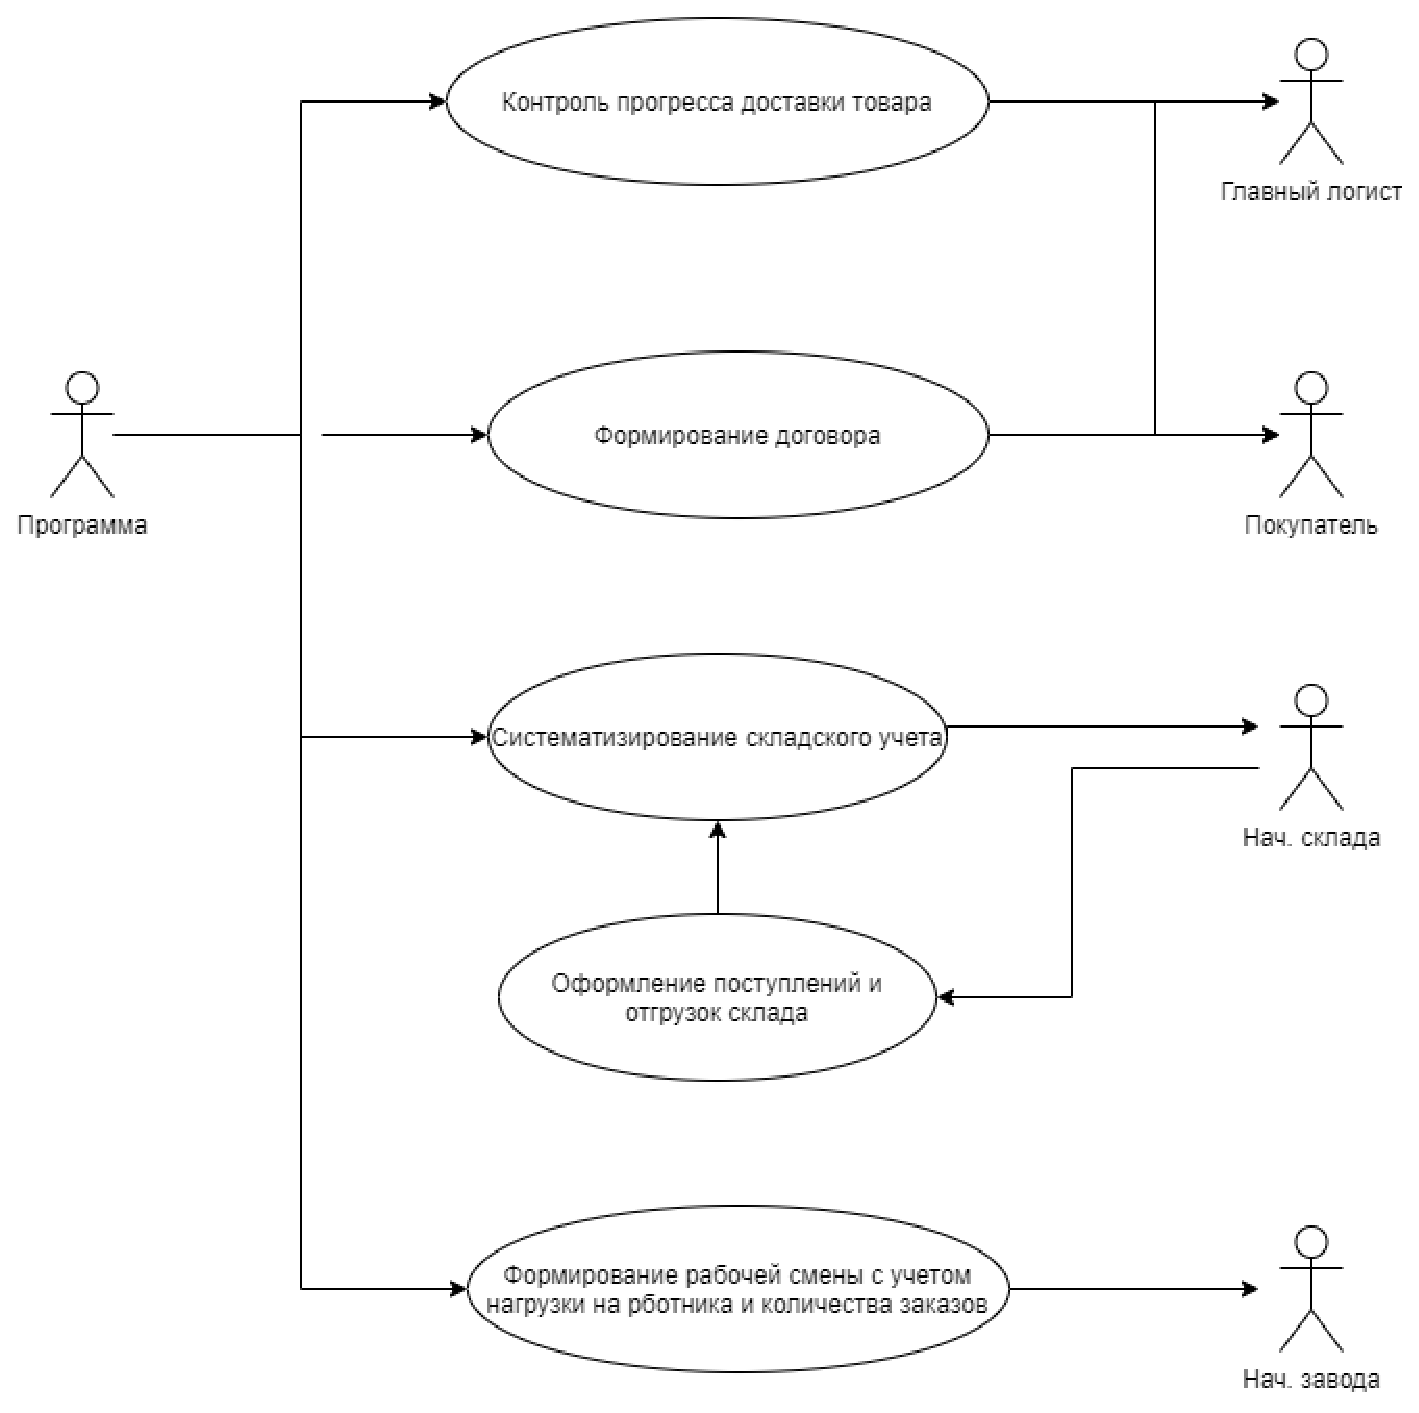
\includegraphics[width=0.5\textwidth]{images/3/usecase.eps}
        \caption{Use-case диаграмма системы}
\end{figure}

\subsection{Круг заинтересованных лиц}

Таблица 3.5 --- Круг заинтересованных лиц
\begin{table}[h!]
\resizebox{\textwidth}{!}{%
\begin{tabular}{|l|l|}
\hline
Эктор & Уровень 			доступа \\ \hline
Генеральный 			директор & Администратор \\ \hline
Начальник 			завода & Администратор \\ \hline
Начальник 			складского отдела & Администратор \\ \hline
Главный 			бухгалтер & Администратор \\ \hline
Начальник 			смены & Пользователь 			с расширенными возможностями \\ \hline
Главный 			логист & Пользователь 			с расширенными возможностями \\ \hline
Бухгалтеры & Пользователь \\ \hline
Водитель 			фуры & Пользователь \\ \hline
Рабочие & Пользователь \\ \hline
Складской 			работник & Пользователь \\ \hline
\end{tabular}%
}
\end{table}

\subsection{Границы использования системы}

\begin{enumerate}
	\item{Мощности ЭВМ предприятия ограничены, на большинстве ЭВМ сотрудников предприятия установлено проприетарное ПО --- оплата лицензий ПО превышает 5 \% дохода.}

	\item{Временные затраты на разработку зависят от пика продаж строительства на рынке --- программная система дожна быть реализована в период между II и IV кварталом текущего года.}

	\item{Помимо этого, бюджет на разработку ограничен и не может превышать 25000 USD, также средства необходимо направить на обучение работников цифровым навыкам.} 

\end{enumerate}
		\subsection{Основные свойства системы}


Таблица 3.6 --- Основные свойства системы
% Please add the following required packages to your document preamble:
% \usepackage{graphicx}
\begin{table}[h!]
\resizebox{\textwidth}{!}{%
\begin{tabular}{|l|l|l|}
\hline
Бизнес-процесс & Участники & Выгода для предприятия \\ \hline
Оформление 			договора & Бухгалтеры & Уменьшение 			временных затрат на обработку заявок \\ \hline
Отгрузка 			покупателю & Главный 			логист & Уменьшение 			времени согласования и сложности 			контроля процесса доставки \\ \hline
Отгрузка 			покупателю & Водитель 			фуры & Удобное 			формирование графика через ИС \\ \hline
Отгрузка 			на склад & Начальник 			склада & Удобство 			хранения и поиска документов продукта \\ \hline
\end{tabular}%
}
\end{table}

\section{Диаграммы IDEF0 для предметной области}

На рисунках 3.6 и 3.7 представлены диаграммы IDEF0 для предметной области.

\begin{figure}[h!]
        \centering
        \includegraphics[width=0.7\textwidth]{images/3/idef1.eps}
        \caption{Автоматизированная схема объекта}
\end{figure}

\begin{figure}[h!]
        \centering
        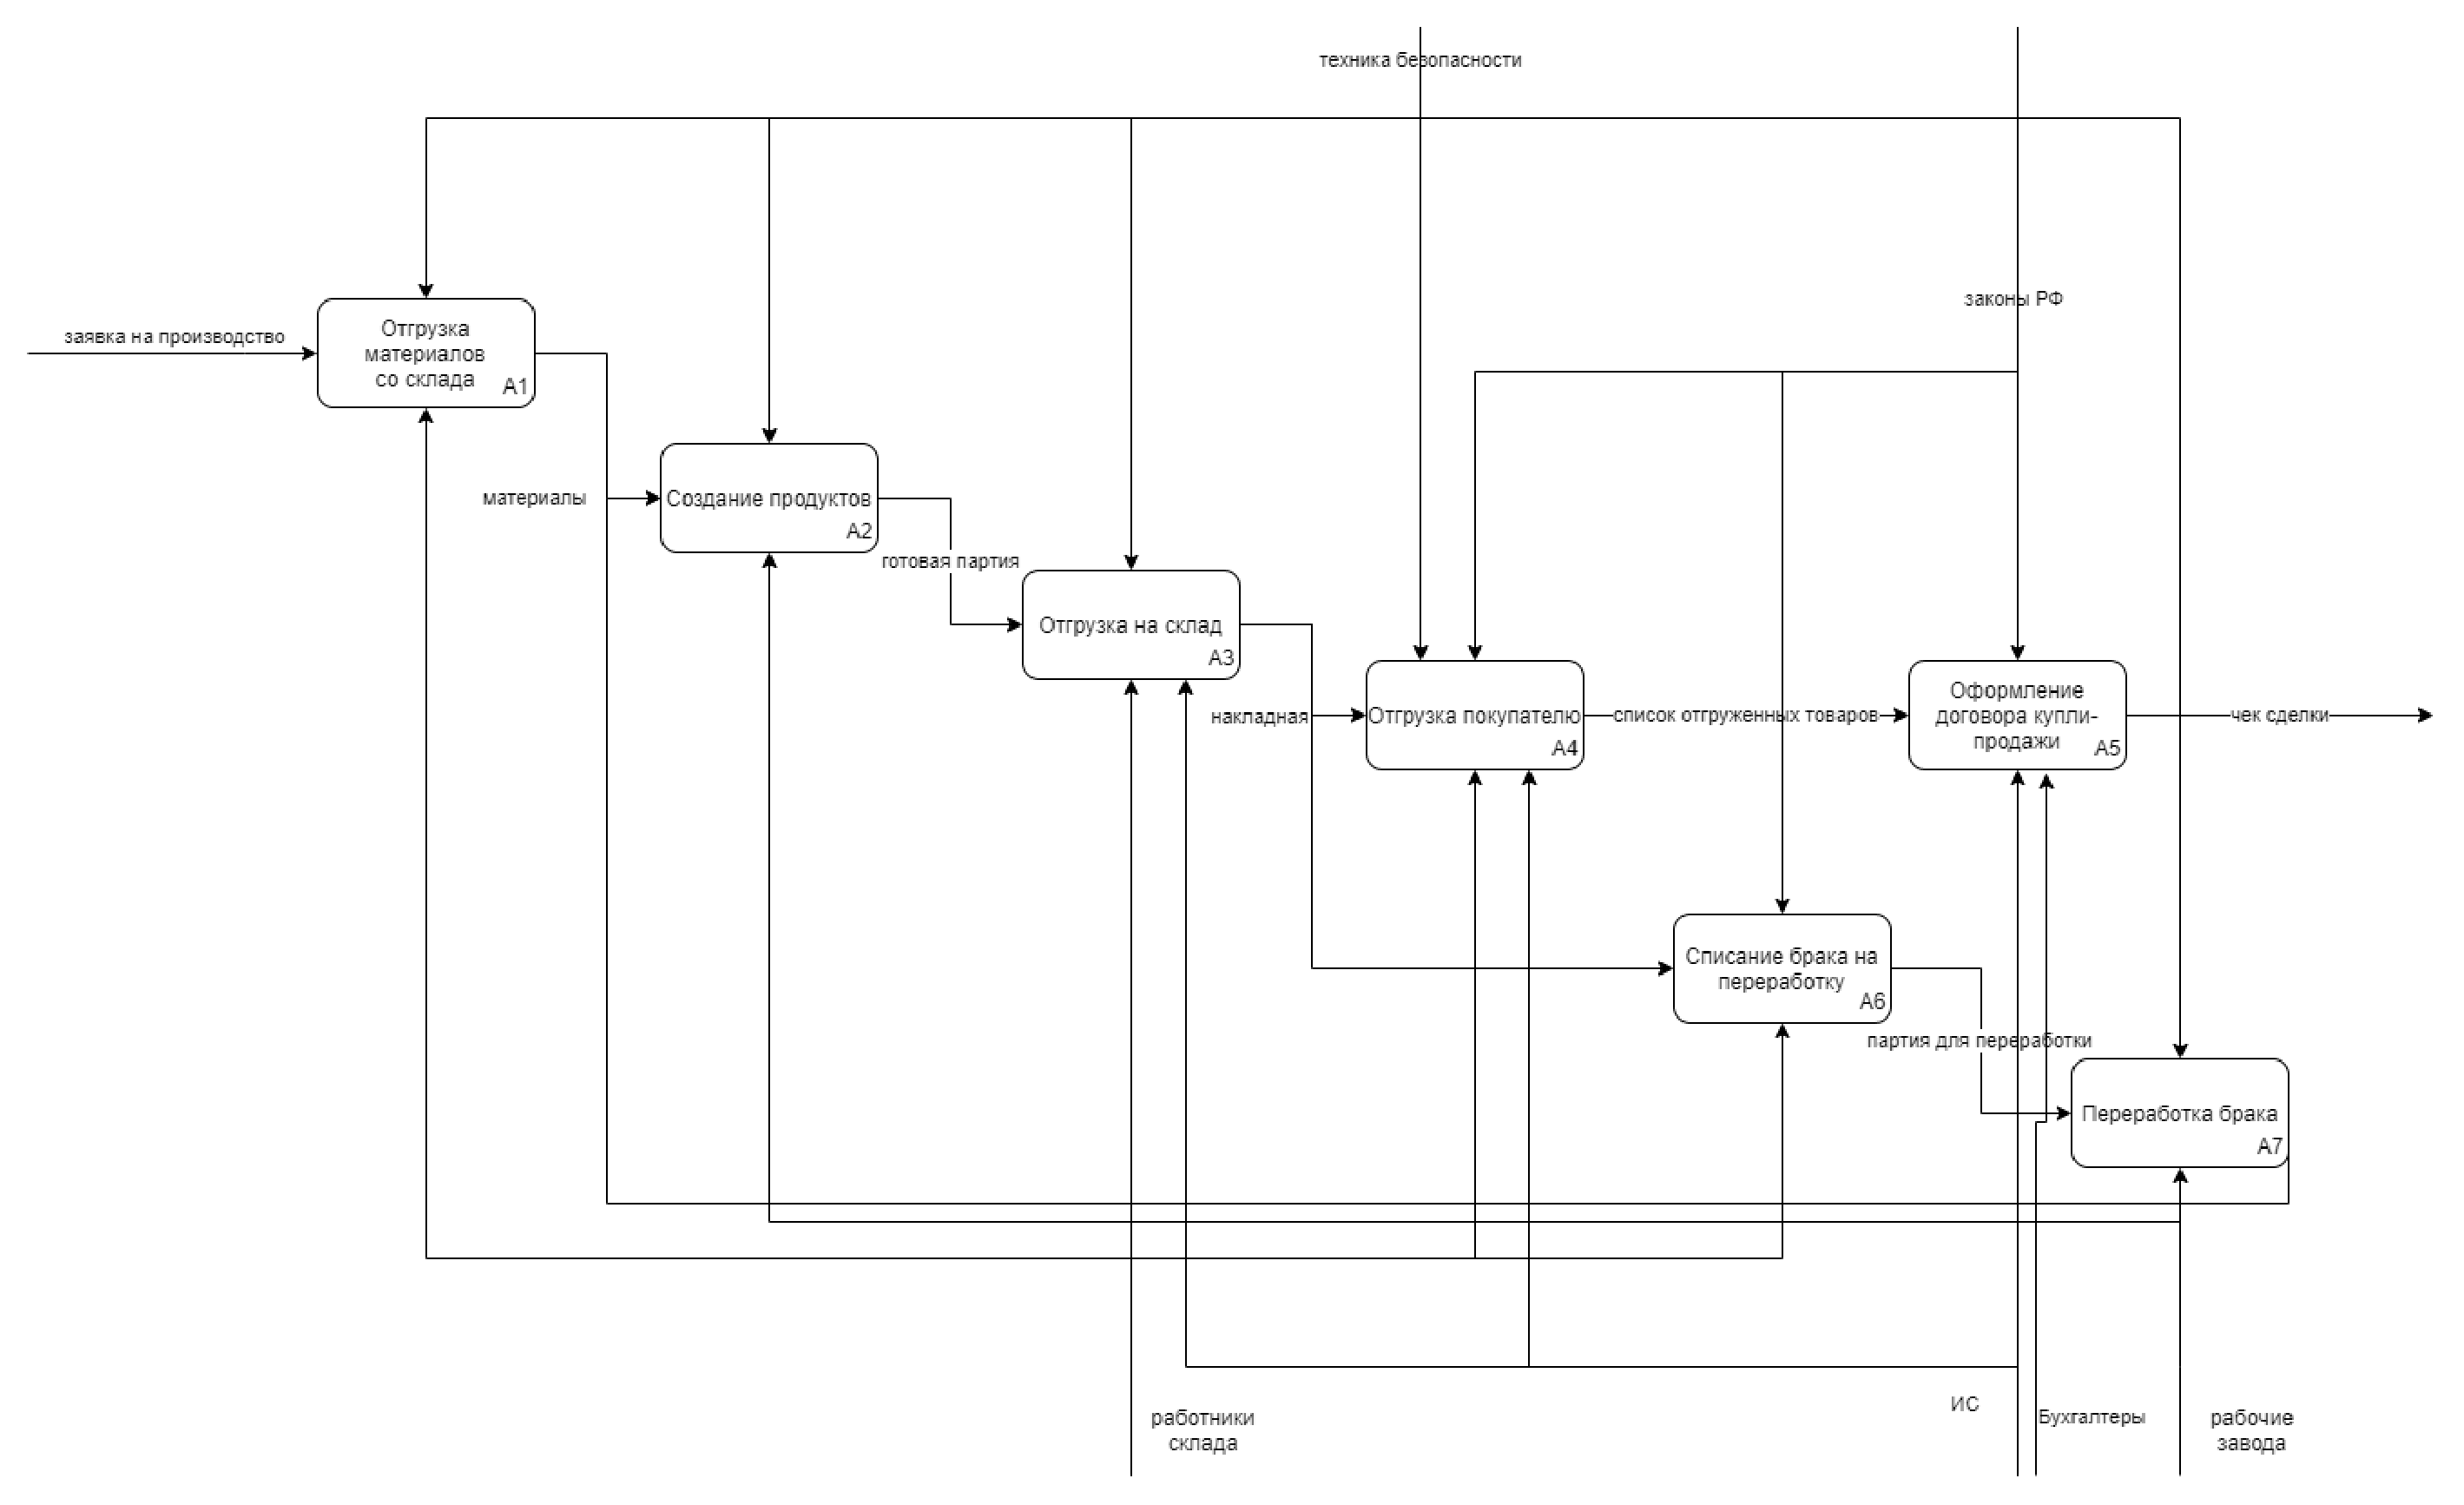
\includegraphics[width=0.7\textwidth]{images/3/idef2.eps}
        \caption{Автоматизированная схема объекта}
\end{figure}

\section{Заключение}

В результате выполнения практической работы были получены навыки использования методологии функционального моделирования IDEF0, построены функциональные модели на основании требований к информационной системе агентства недвижимости. В процессе работы было выполнено обследование объекта автоматизации, составление обоснования необходимости информационной системы, выполнен анализ рисков и составлен аналитический отчет по проектированию информационной системы. 
